% Geometric Quantum States
%
% fa: 4/31/20, 5/4/20
% jpc: 5/1/20, 5/6/20

\documentclass[draft,nofootinbib,prl,twocolumn,showpacs,showkeys,groupaddress,preprintnumbers,floatfix]{revtex4-1}
%\documentclass[nofootinbib,pre,twocolumn,showpacs,showkeys,groupaddress,preprintnumbers,floatfix]{revtex4-1}

\usepackage{dynlearn}
\usepackage{physics}

% \usepackage[utf8]{inputenc}
\usepackage{mathrsfs}
\usepackage[english]{babel}
\usepackage{amssymb,amscd}
\newtheorem{theorem}{Theorem}
\newtheorem{hypothesis}{Hypothesis}

% \newcommand{\norm}[1]{\left\Vert#1\right\Vert}
% \newcommand{\abs}[1]{\left\vert#1\right\vert}
% \newcommand{\set}[1]{\left\{#1\right\}}
% \newcommand{\R}{\mathbb{R}}
\newcommand{\e}{\mathrm{e}}
\newcommand{\Hilb}{\mathcal{H}}
\newcommand{\eps}{\varepsilon}
\newcommand{\To}{\longrightarrow}
\newcommand{\BX}{\mathbf{B}(X)}
\newcommand{\A}{\mathcal{A}}
\newcommand{\HH}{\Hilb}
\newcommand{\g}{\mathfrak{g}}
\newcommand{\Ug}{\mathcal{U}\mathfrak{g}}
\newcommand{\Tg}{\mathcal{T}\mathfrak{g}}
\newcommand{\Sg}{\mathcal{S}\mathfrak{g}}
\newcommand{\Us}{\mathcal{U}\mathfrak{s}}
\newcommand{\Ss}{\mathcal{S}\mathfrak{s}}
% \DeclareMathOperator{\Tr}{Tr}
\DeclareMathOperator*{\argmax}{arg\,max}
\DeclareMathOperator*{\argmin}{arg\,min}
\newcommand{\Ut}[1]{\undertilde{#1}}
\newcommand{\1}{\mathbbm{1}}
\newcommand{\circled}[1]{\tikz[baseline=(C.base)]\node[draw,circle,inner sep=1. 2pt,line width=0.2mm,](C) {\small #1};\!}
\newcommand{\Pexp}[1]{\mathrm{Pexp} \left[ #1 \right] }
\newcommand{\Ch}[1]{ \mathrm{Ch} \; #1}
\newcommand{\Sh}[1]{ \mathrm{Sh} \; #1}
% \newcommand{\Ket}[1]{ \left| #1 \right\rangle}
% \newcommand{\Bra}[1]{ \left\langle #1 \right|}
\newcommand{\Scal}[2]{ \left\langle #1 | #2 \right\rangle}
\newcommand{\KetQ}[1]{ \left| #1 \right]}
\newcommand{\BraQ}[1]{ \left[ #1 \right|}
\newcommand{\ScalQ}[2]{ \left[ #1 | #2 \right]}
\newcommand{\Miss}[2]{ \left[ #1 | #2 \right\rangle}
\newcommand{\MissQ}[2]{ \left\langle #1 | #2 \right]}
\newcommand{\ZT}{\undertilde{z}}
\newcommand{\Z}{\zeta}
\newcommand{\MV}[1]{\left\langle #1 \right\rangle}
\newcommand{\MC}[1]{\left\langle #1 \right\rangle_{\mathrm{mc}}}
% \newcommand{\braket}[2]{\langle #1 | #2 \rangle}
% \newcommand{\ketbra}[2]{| #2 \rangle\langle #1 |}
% \newcommand{\ket}[1]{| #1 \rangle}
% \newcommand{\bra}[1]{\langle #1 |}
\renewcommand{\equiv}{\coloneqq}
\newcommand{\PP}[4]{\mathbin{_{#2} P^{#1}_{#3}} \left[ #4 \right]}
\newcommand{\intP}{\int_{\mathcal{P}(\mathcal{H})} \!\!\!\!\!\!\!\!\!}
\newcommand{\intPB}{\int_{\mathcal{P}(\overline{\mathcal{H}})} \!\!\!\!\!\!\!\! \!}
\newcommand{\PH}{\mathcal{P}(\mathcal{H})}

\def\d{\delta}
\def\f{\frac}
\def\om{\omega}
\def\w{\wedge}
\def\la{\langle}
\def\ra{\rangle}
\newcommand{\p}{\partial}
\newcommand{\n}{\nabla}

\newcommand{\cg}[1]{{\color{blue}[[CG: #1]]}}
\newcommand{\fa}[1]{{\color{red}[[FA: #1]]}}
\newcommand{\cut}[1]{{\color{purple}[[CUT?: #1]]}}

\newenvironment{entry}
  {\begin{list}{--}{
      \setlength{\topsep}{0pt}
      \setlength{\itemsep}{0pt}
      \setlength{\parsep}{0pt}
      \setlength{\labelwidth}{5pt}
      \setlength{\itemindent}{0pt}}}{\end{list}}

\def\tbf #1 {\textbf{#1} }

\begin{document}

\def\ourTitle{%
Geometric Quantum States
}

\def\ourAbstract{%
A quantum system's state is often identified with a density matrix. Though
their probabilistic interpretation is rooted in ensemble theory, density
matrices embody a known shortcoming. They do not completely express the
physical realization of an ensemble. Fortunately, when working only with the
statistical outcomes of positive-operator values measurements (POVMs) this is
not a hindrance. Here we explore the notion of geometric quantum state, as a
way to keep track of the ensemble realization, and its physical relevance.  
We emphasize two main perspectives: quantum control and quantum thermodynamics.
{\bf HERE}
Its geometric quantum states are complete and, if
needed, the density matrix description can be extracted from them.
}

\def\ourKeywords{%
Quantum Mechanics, Geometric Quantum Mechanics
}

\hypersetup{
  pdfauthor={Fabio Anza},
  pdftitle={\ourTitle},
  pdfsubject={\ourAbstract},
  pdfkeywords={\ourKeywords},
  pdfproducer={},
  pdfcreator={}
}

%%%%%%%%%%%%%%%%%%%%%%%%%%%%%%%%%%%%%%%%%%%%%%%%%%%%%%%%%%%%%%%%%%%%%%%%%%%%%%%

\title{\ourTitle}

\author{Fabio Anza}
\email{fanza@ucdavis.edu}

\author{James P. Crutchfield}
\email{chaos@ucdavis.edu}

\affiliation{Complexity Sciences Center and Physics Department,
University of California at Davis, One Shields Avenue, Davis, CA 95616}

\date{\today}
\bibliographystyle{unsrt}

\begin{abstract}
\ourAbstract
\end{abstract}

\keywords{\ourKeywords}

\pacs{
05.45.-a  %  Nonlinear dynamics and nonlinear dynamical systems
89.75.Kd  %  Complex Systems: Patterns
89.70.+c  %  Information science
05.45.Tp  %  Time series analysis
%02.50.Ey  %  Stochastic processes
%02.50.-r  %  Probability theory, stochastic processes, and statistics
%02.50.Ga  %  Markov processes
%%%%%%%FROM HERE%%%%%%
%05.20.-y  %  Classical statistical mechanics
%02.40.−k %Geometry, differential geometry, and topology
%03.65.−w %Quantum mechanics
%03.67.−a %Quantum information
%05.30.−d %Quantum statistical mechanics
%05.70.−a %Thermodynamics
%%%%%%%TO HERE%%%%%%
}

\preprint{\arxiv{2005.XXXXX}}

\date{\today}
\maketitle

% \tableofcontents

% \setstretch{1.1}

% Collides with table of contents formatting
% \listoffixmes

% {\bf Lead Paragraph:
% }

Quantum mechanics is firmly rooted in a vector formalism where a system's
states $\ket{\psi}$ are elements of a complex Hilbert space $\mathcal{H}$.
These are the system's \emph{pure states}---as opposed to \emph{mixed
states}---that account for incomplete knowledge of a system's actual state. One
transforms states in $\mathcal{H}$ using density matrices $\rho$, operators
that are positive semi-definite $\rho \geq 0$, self-adjoint $\rho =
\rho^\dagger$, and normalized $\Tr \rho = 1$. The interpretation of a density
matrix as a system's \emph{probabilistic state} is given by \emph{ensemble
theory} \cite{Pathria2011,Greiner1995}. Accordingly, since a density matrix
always decomposes into eigenvalues $\lambda_i$ and eigenvectors
$\ket{\lambda_i}$:
\begin{align*}
\rho = \sum_i \lambda_i \ket{\lambda_i}\bra{\lambda_i}
  ~,
\end{align*}
one interprets $\rho$ as an ensemble of pure states---the eigenvectors---in
which $\lambda_i$ is the probability of an observer interacting with
$\ket{\lambda_i}$.

However, this interpretation is problematic: It is not unique. One can write
the same $\rho$ using different decompositions:
\begin{align*}
\rho = \sum_k p_k \ket{\psi_k}\bra{\psi_k}
\end{align*}
that, nonetheless, all identify the same quantum state. While one often prefers
the diagonal decomposition in terms of eigenvalues and eigenvectors, this is
not the only possible decomposition. More tellingly, in principle, there is no
experimental reason to prefer it to other decompositions. In quantum mechanics,
this fact is often addressed by declaring density matrices with the same
barycenter equal. A familiar example of this degeneracy is that the maximally
mixed state has an infinite number of identical decompositions, each possibly
being a distinct ensemble.

\jpcnote{Need a short definition of mixed state above so that maximally-mixed
makes at least intuitive understanding here in the Introduction.}

Moreover, it is rather straightforward to imagine systems that, despite
having the same density matrix, are in a different state. For example, consider
two distinct state-preparation protocols: in one case, prepare states
$\{\ket{0},\ket{1}\}$ each with probability $1/2$ while, in the other case,
always prepare states $\{\ket{-},\ket{+}\}$ each with probability $1/2$. A
complete and unambiguous mathematical characterization of the notion of 
state should not conflate these distinct physical configurations.

So, here we argue that the geometric formalism, together with an appropriately
formulated measure theory, allows to separate between the primary notion of 
\emph{state of the system} and the derived notion of density matrix as the set of 
all \emph{POVM statistics} on that system. 

With this perspective in mind, we introduce a more incisive description of
pure-state ensembles. The following argues that \emph{geometric quantum
mechanics} (GQM), with its notion of \emph{geometric quantum states}, cleanly
resolves the ambiguities. First, we introduce GQM. Second, we discuss how it
relates to the more familiar density matrix formalism and how it handles
outcomes of quantum measurements. Third, {\bf WHAT?}.

\paragraph*{Geometric quantum mechanics.}\label{sec:GQM}
References
\cite{STROCCHI1966,Kibble1979,Heslot1985,Gibbons1992,Ashtekar1995,Ashtekar1999,Brody2001,Bengtsson2017,Carinena2007,Chruscinski2006,Marmo2010,Avron2020,Pastorello2015,Pastorello2015a,Pastorello2016,Clemente-Gallardo2013}
give a comprehensive introduction to GQM. Here, we briefly summarize only the
elements we need, working with Hilbert spaces $\mathcal{H}$ of finite dimension $D$.

Pure states are points in the complex projective manifold $\mathcal{P}\left(
\mathcal{H} \right)=\mathbb{C}\mathrm{P}^{D-1}$. Therefore, given an arbitrary
basis $\left\{\ket{e_\alpha} \right\}_{\alpha=0}^{D-1}$, a pure state $\psi$ is
parametrized by $D$ complex homogeneous coordinates $Z = \left\{      Z^\alpha\right\}$, up to
normalization and an overall phase:
\begin{align*}
\ket{\psi} = \sum_{\alpha=0}^{D-1} Z^\alpha \ket{e_\alpha}
  ~,
\end{align*}
where $Z \in \mathbb{C}^{D}$, $Z \sim \lambda Z$, and $\lambda \in
\mathbb{C}/\left\{ 0\right\}$. If the system consists of a single qubit, for
example, we have $Z = (\sqrt{p_0}e^{i\nu_0},\sqrt{p_1} e^{i\nu_1})$.

An \emph{observable} is a
quadratic real function $\mathcal{O}(Z) \in \mathbb{R}$ that associates to each
point of $\mathcal{P}(\mathcal{H})$ the expectation value $\bra{\psi}
\mathcal{O} \ket{\psi}$ of the corresponding operator $\mathcal{O}$ on
state $Z$:
\begin{align}
\mathcal{O}(Z) = \sum_{\alpha,\beta} \mathcal{O}_{\alpha,\beta}Z^\alpha \overline{Z}^\beta
  ~,
\label{eq:GQM_Observable}
\end{align}
with $\mathcal{O}_{\beta,\alpha} = \overline{\mathcal{O}}_{\alpha,\beta}$.

The probabilities of measurement outcomes are given by \emph{positive
operator-valued measurements} (POVMs) $\left\{E_j\right\}_{j=1}^n$. They are
nonnegative operators $E_j\geq 0$, called \emph{effects}, that sum up to the
identity: $\sum_{j=1}^n E_j = \mathbb{I}$. In GQM they are a collection of
nonnegative real functions $E_j(Z)\ge 0$ on $\mathcal{P}(\mathcal{H})$ whose
sum is always equal to one:
\begin{align}
E_j(Z) = \sum_{\alpha,\beta}
  \left(E_j\right)_{\alpha,\beta} Z^\alpha \overline{Z}^\beta
  ~,
\label{eq:GQM_POVMs}
\end{align}
where $\sum_{j=1}^{n}E_j(Z) = 1$.

Complex projective spaces, such as $\mathcal{P}(\mathcal{H})$, have a preferred
metric $g_{FS}$---the \emph{Fubini-Study metric} \cite{Bengtsson2017}---and an
associated volume element that is coordinate-independent and invariant under
unitary changes. This is the Fubini-Study volume element, which we denote
$dV_{FS}$. The geometric derivation of $dV_{FS}$ is beyond our immediate goals
here. That said, it is sufficient to give its explicit form in the
``probability + phases'' coordinate system ($Z^{\alpha} =
\sqrt{p_\alpha}e^{i\nu_\alpha}$) that we will use for concrete calculations:
\begin{align*}
dV_{FS} & = \sqrt{\det g_{FS}}
  \prod_{\alpha=0}^{D-1} dZ^\alpha d\overline{Z}^\alpha \\
  & =  \prod_{\alpha=1}^{D-1} \frac{dp_\alpha d\nu_\alpha}{2}
  ~.
\end{align*}
Notice, here, how $p_0$ and $\nu_0$ are not involved. This is due to
$\mathcal{P}(\mathcal{H})$'s projective nature which guarantees that we can
choose a coordinate patch in which $p_0 = 1 - \sum_{\alpha=1}^{D-1}p_\alpha$
and $\nu_0 = 0$.

\paragraph*{Geometric quantum states.}
This framework makes it very natural to view a quantum state as a functional
encoding that associates expectation values to observables, as done in the
$C^{*}$-algebras formulation of quantum mechanics \cite{Strocchi2008a}. Thus,
states can be described via functionals $P[\mathcal{O}]$ from the algebra of
observables $\mathcal{A}$ to the real line: 
\begin{align*}
P_p[\mathcal{O}]
  = \int_{\mathcal{P}(\mathcal{H})} p(Z) \mathcal{O}(Z) dV_{FS}
  ~,
\end{align*}
where $\mathcal{O} \in \mathcal{A}$, $p(Z) \geq 0$ is the
normalized distribution associated with functional $P$:
\begin{align*}
P_p[\mathbb{I}] = \int_{\mathcal{P}(\mathcal{H})}
  p(Z) dV_{FS}  = 1
  ~,
\end{align*}
and $P_p[\mathcal{O}] \in \mathbb{R}$.

In this way, pure states $\ket{\psi_0}$ are functionals with a Dirac-delta-like
distribution $p_0(Z) = \widetilde{\delta}\left[ Z - Z_0\right]$:
\begin{align*}
P_{0}[\mathcal{O}] &= \intP \widetilde{\delta}(Z-Z_0)\mathcal{O}(Z) dV_{FS} \\
  & = \mathcal{O}(Z_0)  = \bra{\psi_0}\mathcal{O}\ket{\psi_0}
  ~.
\end{align*}
$\widetilde{\delta}(Z-Z_0)$ is shorthand for a coordinate-covariant Dirac-delta in
arbitrary coordinates. In homogeneous coordinates this reads:
\begin{align*}
\widetilde{\delta}(Z - Z_0) \coloneqq \frac{1}{\sqrt{\det g_{FS}}}
  \prod_{\alpha=0}^{D-1} \delta(X - X_0) \delta(Y - Y_0)
  ~,
\end{align*}
where $Z = X + iY$. In $(p_\alpha,\nu_\alpha)$ coordinates this becomes simply:
\begin{equation}
\widetilde{\delta}(Z - Z_0) = \prod_{\alpha=1}^{D-1} 2\delta(p_\alpha - p_\alpha^0) \delta(\nu_\alpha - \nu_\alpha^0)
  ~,
\end{equation}
where the coordinate-invariant nature of the functionals $P_p[\mathcal{O}]$ is
now apparent.

In this way, too, mixed states:
\begin{align*}
\rho = \sum_{j}\lambda_j \ket{\lambda_j}\bra{\lambda_j}
\end{align*}
are convex combinations of these Dirac-delta-like functionals:
\begin{align*}
p_{\mathrm{mix}}(Z) = \sum_{j}\lambda_j \widetilde{\delta}(Z-Z_j)
  ~. 
\end{align*}
Thus, the mixed states expressed as functionals from observables to the real
line are:
\begin{align}
P_{\mathrm{mix}}\left[ \mathcal{O}\right]
  & = \sum_{j} \lambda_j \bra{\lambda_j}\mathcal{O}\ket{\lambda_j}
  ~.
\label{eq:Functional}
\end{align}

Equipped with this formalism, one identifies the distribution $p(Z)$ as a
system's \emph{geometric quantum state}. This is the generalized notion of
quantum state we are interested in.

A simple example of an ensemble that is neither a pure nor a mixed state is
the \emph{geometric canonical state}:
\begin{align*}
p(Z) = \frac{1}{Q_\beta} e^{-\beta h(Z)}
  ~,
\end{align*}
where:
\begin{align*}
  Q_\beta & = \int dV_{FS} e^{-\beta h(Z)} ~, \\
  h(Z) & = \bra{\psi(Z)}H\ket{\psi(Z)} ~,
\end{align*}
and $H$ is the system's Hamiltonian operator. This state was previously
considered in Refs. \cite{Brody1998,Brody2016}. Reference \cite{Anza20a}
investigated its potential role in establishing a quantum foundation of
thermodynamics that is an alternative to that based on Gibbs ensembles and von
Neumann entropy. Moreover, it was shown in Ref.\cite{Anza20a} that such ensemble
is genuinely different from Gibbs ensemble, providing an experimental venue to 
test the experimental relevance of the geometric quantum state.


\paragraph*{Density matrix.}
The connection between geometric quantum states and density matrices is
two-fold. On the one hand, when the distribution $p(Z)$ falls into one of the
two aforementioned cases---Dirac-deltas or finite convex combinations of
them---the present formalism is equivalent to the standard one. However, not
all functionals are of these simple Dirac-delta-like form. Thus, $p(Z)$ is
clearly a more general notion of state of a quantum system.

On the other hand, given an arbitrary distribution $p(Z)$, there is a unique
density matrix $\rho^{p}$ associated to $p$:
\begin{align}
\rho^p_{\alpha \beta} & = P_p[Z^\alpha \overline{Z}^\beta] \nonumber \\
  & = \intP dV_{FS} \, p(Z)  \, Z^\alpha \overline{Z}^\beta
  ~.
\label{eq:densitymatrix}
\end{align}
Owing it to the fact that all POVMs are represented by real and quadratic
functions on $\mathcal{P}(\mathcal{H})$, recall Eq. (\ref{eq:GQM_POVMs}), they
are not directly sensitive to $p(Z)$, but only to $\rho^p$. Therefore, if two
distributions $p_1$ and $p_2$ induce the same density matrix $\rho^{p_1} =
\rho^{p_2}$, then all POVMs produce the same outcomes.

A well-known consequence of this fact is that two density matrices with the
same barycenter are considered equal, even if they describe experiments with
different physical configurations. In these cases, the statistics of POVM
outcomes are described by the same density matrix. While this statement means
that without further processing there is no POVM on the system that can distinguish 
between $p_1$ and $p_2$, it does not mean that there is no possible observable
difference, as we explicitly demonstrate in the following. 

We believe that this is particularly important for information processing
tasks---as encountered in quantum computing, for example---in which one is not
only interested in measurement outcomes, but also in understanding, predicting,
and controlling how a quantum system responds to external manipulations. For the
same reason, this formalism appears to emerge naturally in a quantum thermodynamics
context, as argued in Ref.\cite{Anza20a}.\\

%In such settings, understanding whether a
%state-preparation protocol produces Dirac-delta-like distributions of pure
%states or more general distributions is paramount to properly address
%computational errors and to analyzing the thermodynamic costs of quantum
%computation.

\paragraph*{Distinguishability.}\label{sec:distinguishability}
Conventionally, two density matrices with the same barycenter are effectively
equal. Due to this, one cannot distinguish two different physical
configurations described by density matrices with the same barycenter. On the
flip side, a given density matrix decomposes into distinct pure-state
ensembles. Experimentally, such ensembles cannot be distinguished using the
measurement statistics extracted via POVMs.

While this is all correct and familiar, we now demonstrate that it is, in fact,
possible to distinguish these ensembles. The following gives a concrete
scenario that clarifies how geometric quantum mechanics circumvents the
information loss implicit in density matrix descriptions of quantum states. The
result is a more accurate and complete theoretical description of a quantum
experiment.

The scenario mimics a state-preparation protocol followed by state
manipulation. There are two classical operators: Alice and Bob. Alice has a
biased coin $\left\{ H,T\right\}$, with $p_A(H) = (1+\lambda)/2$ and $p_A(T) =
(1-\lambda)/2$, and two bags of qubit pure states. The first bag contains
identical copies of $\ket{0}$, while the second contains identical copies of
its orthogonal state $\ket{1}$. Each time she throws the coin, if Alice
observes $H$ she grabs a state from the first bag, otherwise she samples from
the other. The result of this process is a state ensemble described by the
density matrix:
\begin{align}
\rho_A & = p_A(H) \ket{0}\bra{0} + p_A(T) \ket{1}\bra{1} \nonumber \\
  & = \frac{1}{2}\left( \mathbb{I} + \lambda \sigma_z \right)
  ~.
\label{eq:rhoA} 
\end{align}
To refine notation let $\ket{\psi_H^A} = \ket{0}$ and $\ket{\psi_T^A} =
\ket{1}$.

Now, Bob is aware of Alice's classical bias $\lambda$ and is interested in 
reproducing Alice's outcome. However, since he wants to experiment with quantum
mechanics, he decides to stick to fair coins $p_B(H)=p_B(T)= \frac{1}{2}$, but
uses quantum states with an overlap identical to the classical bias:
\begin{subequations}
\begin{align}
\ket{\psi_H^B} & = \sqrt{\frac{1+\lambda}{2}} \ket{0} +
\sqrt{\frac{1-\lambda}{2}} e^{i\chi} \ket{1}~\text{and}\\
\ket{\psi_T^B} & = \sqrt{\frac{1+\lambda}{2}} \ket{0} - \sqrt{\frac{1-\lambda}{2}} e^{i\chi}\ket{1}
  ~.
\end{align}
\end{subequations}
Here, $\chi \in [0,2\pi]$ is arbitrary and all states are legitimate quantum states that Bob can use.

Alice's bias $p_A(H)-p_A(T) = \lambda$ is the same as the \emph{fidelity}:
\begin{align*}
|\braket{\psi_H^B}{\psi_T^B}|^2 = \lambda
  ~.
\end{align*}
Thus, Bob's experiment is described by the density matrix:
\begin{align*}
\rho_B = p_B(H) \ket{\psi_H^B}\bra{\psi_H^B}
  + p_B(T) \ket{\psi_T^B}\bra{\psi_T^B} 
  ~.
\end{align*}
By inspection one sees that Alice's an Bob's protocols give the same density
matrix:
\begin{align*}
\rho_A  & = \rho_B \\
  & = \frac{1}{2}\left( \mathbb{I} + \lambda \sigma_z\right) \\
  & = \left( \begin{array}{cc}
  \frac{1+\lambda}{2} & 0 \\ 0 & \frac{1-\lambda}{2}
  \end{array} \right)
~.
\end{align*}

\begin{figure}[h]
\centering
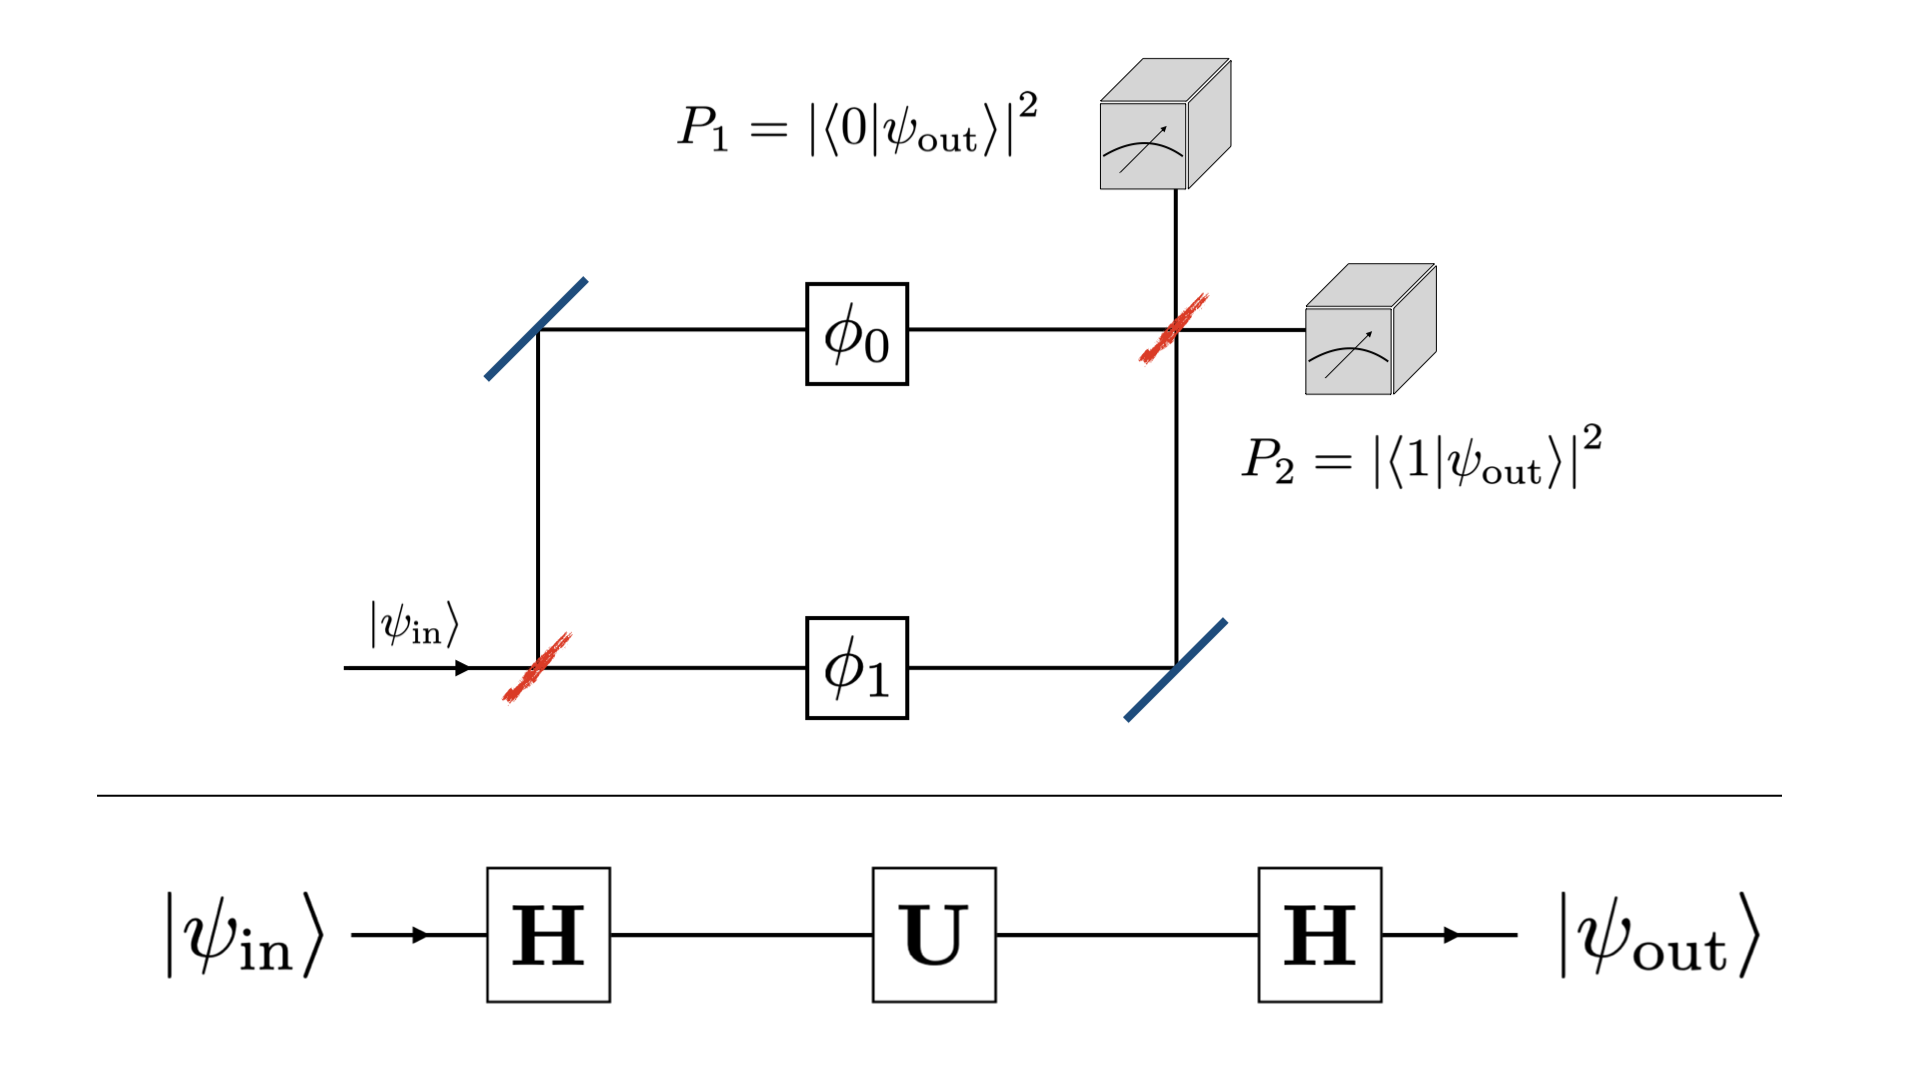
\includegraphics[width=.9\columnwidth]{img/InterferometerCircuit.png}
\caption{Interferometric detection scheme (upper) with its circuit
	representation (lower). An input state $\ket{\psi_{\mathrm{in}}}$ passes
	through a beam splitter (left diagonal red line), reflects off two mirrors
	(blue diagonal lines), undergoes a phase-shift, with phase $\phi_0$ in the
	upper path and $\phi_1$ in the lower path, and eventually passes through a
	second beam splitter (right diagonal red line), and hits either detector
	$1$ or $2$. (We assume mirrors do not modify the system's state.)
	}
\label{fig:interferometer} 
\end{figure}

Stepping back, shifting from Alice to Bob trades a classical source (Alice's)
of randomness for one (Bob's) of quantum nature. However, invoking standard
quantum mechanics, having the same density matrix one must conclude that there
is no observable difference between the two protocols. In practice, this
translates into the fact that the results of a quantum tomography protocol
yield the same answer. Moreover, again by standard quantum mechanics, if we
perform an information-processing task and then perform a measurement, we
conclude that there is no discernible difference between the results of Alice's
and Bob's protocols.

When the states resulting from both state-preparation protocols pass through an
interferometer, as depicted in Fig. \ref{fig:interferometer}(upper), we model
the output with the unitary operator $M = HUH$, where $H$ is the Hadamard gate
describing a beam-splitter:
\begin{align*}
H & = \frac{1}{\sqrt{2}}
  \left( \begin{array}{cc}
  1 & 1 \\1 & -1
  \end{array} \right) \\
\end{align*}
and $U$ is a phase-shift:
\begin{align*}
U & = \left( \begin{array}{cc}
  e^{i\phi_0} & 0 \\ 0 & e^{i\phi_1}
  \end{array} \right)
  ~,
\end{align*}
from which only the difference $\phi_0-\phi_1$ is observable. The
interferometer is represented with the simple quantum circuit in Fig.
\ref{fig:interferometer}(lower).

The statistics of the two detectors performing measurement in the computational basis is given by:
\begin{align*}
P_1^{(A)} & = \bra{0}M \rho_A M^\dagger \ket{0} ~,\\
P_2^{(A)} & = \bra{1}M \rho_A M^\dagger \ket{1} ~,\\
P_1^{(B)} & = \bra{0}M \rho_B M^\dagger \ket{0} ~,~\text{and}\\
P_2^{(B)} & = \bra{1}M \rho_B M^\dagger \ket{1}
  ~.
\end{align*}
Since $\rho_A = \rho_B$ we conclude that $P_i^{(A)} = P_i^{(B)}$, with:
\begin{subequations}
\begin{align}
P_1^{(A)} & =
  \frac{1}{2} + \frac{\lambda}{2}\cos (\phi_0 - \phi_1) ~\text{and} \\
P_2^{(A)} & = 1 - P_1^{(A)}
  ~.
\end{align}
\label{eq:expected_result}
\end{subequations}

\begin{figure}[H]
\centering
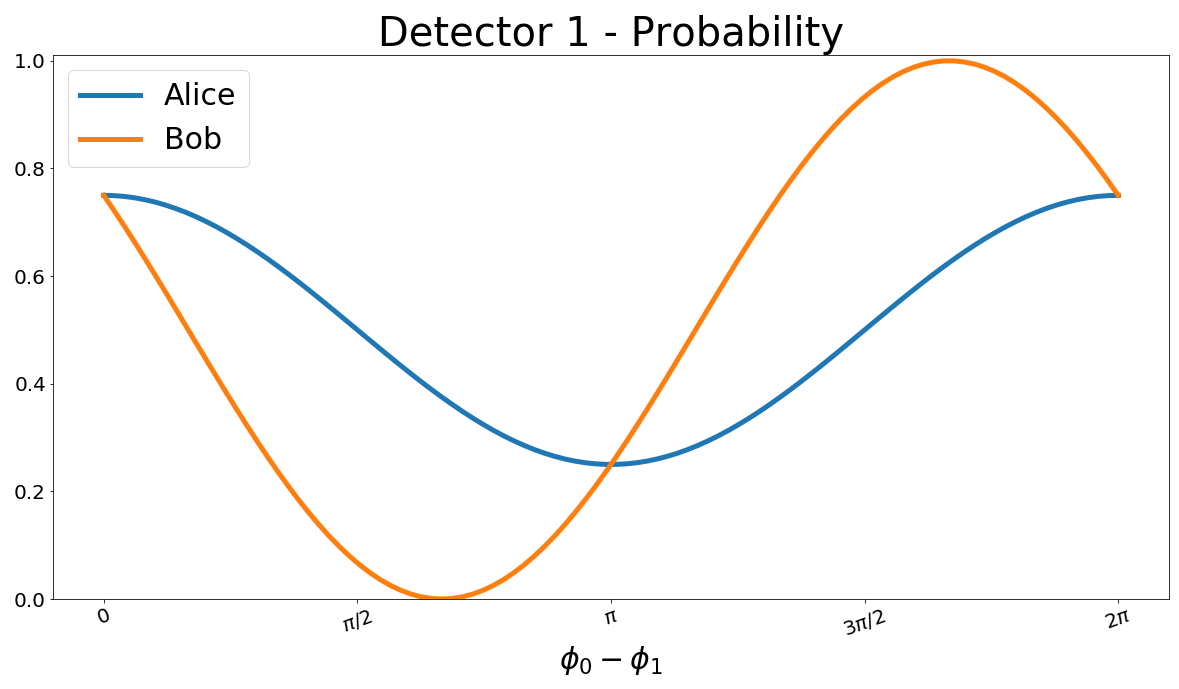
\includegraphics[width=.9\columnwidth]{img/Distinguishability.png}
\caption{Probability of observing an event in detector $1$ as a function of
	the phase-shift $\phi_0 - \phi_1$. Alice (blue) and Bob (orange) protocol
	results are given by Eq. (\ref{eq:expected_result}) and Eq.
	(\ref{eq:new_result}), respectively. Here, $\lambda = 0.5$ and $\chi =
	\frac{\pi}{2}$.
	}
\label{fig:distinguishability} 
\end{figure}

However, if instead of the description $\rho = \frac{1}{2}\left(
\mathbb{I}+\lambda \sigma_z\right)$, use that of the geometric quantum state
or, for that matter, the $\rho_B$ functional form, differences between Alice
and Bob arise. Calling $q_A(Z)$ and $q_B(Z)$ the probability distribution on
$\mathcal{P}(\mathcal{H})$ describing Alice's and Bob's states after they pass
through the interferometer, respectively, one finds:
\begin{subequations}
\begin{align}
q_A(Z) & \!=\! p_A(H) \widetilde{\delta}(Z - Z_H^A)
  + p_A(T) \widetilde{\delta}(Z - Z_T^A)
  ~\text{and} \\ 
q_B(Z) & \!=\! p_B(H) \widetilde{\delta}(Z - Z_H^B)
  + p_B(T) \widetilde{\delta}(Z - Z_T^B)
  ~,
\end{align}
\end{subequations}
where $Z_{H(T)}^A$ is such that:
\begin{align*}
\ket{\psi_{H(T)}^A} = \sum_{k=0}^1 \left( Z_{H(T)}^A \right)_k \ket{k}
  ~.
\end{align*}
Similar relations hold for $Z_{H(T)}^B$.

With these geometric quantum states we can compute the probability of a photon
ending up in detectors using the geometric formalism described above. For
detector 1, the results are:
\begin{align*}
\widetilde{P}_1^{(A)} & = p_A(H)\vert\bra{0}M\ket{\psi_H^A}\vert^2
  + p_A(T)\vert\bra{0}M\ket{\psi_T^A}\vert^2 ~\text{and} \\
\widetilde{P}_1^{(B)} & = p_B(H)\vert\bra{0}M\ket{\psi_H^B}\vert^2
  + p_B(T)\vert\bra{0}M\ket{\psi_T^B}\vert^2
  ~.
\end{align*}
This gives the expected result $\widetilde{P}_1^{(A)}
=P_1^{(A)}$ from Eq. (\ref{eq:expected_result}). While for
$\widetilde{P}_1^{(B)}\neq P_1^{(B)}$ one finds:
\begin{align}
\widetilde{P}_1^{(B)} \!=\! \frac{1}{2}
  \!+\! \frac{\lambda}{2} \cos (\phi_0 \!-\!\phi_1)
  \!-\! \sqrt{\frac{1-\lambda^2}{4}} \sin (\phi_0\!-\!\phi_1)
  \sin \chi
  .
\label{eq:new_result}
\end{align}
Figure \ref{fig:distinguishability}'s plots of these probabilities as a
function of phase shift $\phi_0-\phi_1$ clearly reveals the differences between
$\widetilde{P}_1^{(A)} = P_1^{(A)} = P_1^{(B)}$ and $\widetilde{P}_1^{(B)}$.

\paragraph*{Concluding remarks.}
Conventional quantum mechanics harbors a degeneracy caused by the
fact that two physically-distinct ensembles can have the same density matrix,
as Alice and Bob did. Limiting ourselves to the statistics of POVM outcomes,
this is not an issue. Indeed, one can check that the POVM statistics of Alice
and Bob are the same. However, if we use the density matrix $\rho =
\frac{1}{2}\left( \mathbb{I} + \lambda \sigma_z\right)$ to address the
information-processing task described by Fig. \ref{fig:interferometer}'s
circuit, we are misled and arrive at incorrect predictions. This highlights a
serious shortcoming of conventional quantum mechanics: Holding up the density
matrix as the sole descriptor of a system's state brings down on ourselves
the error of ignoring how an ensemble is realized in practice. Most directly,
this has severe consequences when analyzing information-processing tasks that
occur, for example, when a state ensemble passes through a quantum channel.

The geometric formalism provides an elegant, rigorous, and more inclusive
alternative to the standard vector-based formalism of quantum mechanics. Its
geometric quantum state is a probability distribution on the manifold of pure
states and, in needed, density matrices can be computed as quadratic averages
via Eq. (\ref{eq:densitymatrix}). We emphasized a key advantage of the
geometric formalism: It encodes both density matrix information, about all POVM
statistics, and the ensemble realization. As a result, one can distinguish
between different quantum states having the same POVM outcome statistics. This
is particularly germane for quantum information and quantum computation since
the distinct ensemble realizations of a density matrix are key to appropriately
predicting the results of information processing tasks. Moreover, the
alternative is also important for tasks of classical simulations of quantum
phenomena as, inherently, our software largely calculates based on the matrix
representation of a density operator that, again, does not encode the
information about an ensemble's physical realization.

The lessons are simple. While the density matrix correctly captures all
possible POVMs outcome statistics, it is not a complete description of the
``state of the system''. Rather, this role is appropriately played by the
\emph{geometric quantum state}.

\section*{Acknowledgments}
\label{sec:acknowledgments}
FA thanks Davide Pastorello and Davide Girolami for discussions on the
geometric formalism of quantum mechanics. We thank many people ... for helpful
discussions and the Telluride Science Research Center for its hospitality
during visits. This material is based upon work supported by, or in part by, a
Templeton World Charity Foundation Power of Information Fellowship, FQXi
Grant FQXi-RFP-IPW-1902, and U.S. Army Research Laboratory and the U. S. Army
Research Office under contracts W911NF-13-1-0390 and W911NF-18-1-0028.

\bibliography{library}

\end{document}
